\chapter{Implementierung - Pathcompare}
\label{sec:implementierung}
\section{Technischer Rahmen}

\subsection{Robot Operating System - ROS}

Innerhalb des Referenzsystems wird \gls{ROS} im Zusammenhang mit der Steuerung
des Roboters genutzt und um die während einer Testfahrt gewonnenen Pfaddaten
zu übermitteln. Im Folgenden wird genauer auf die Fähigkeiten und
Ziele von ROS eingegangen.

Obwohl der Name zunächst anderes vermuten lässt, ist ROS kein
Betriebssystem im klassischem Sinne. Es ist vielmehr eine Sammlung von
Anwendungen, welche auf ein Betriebssystem angewiesen sind, um ausgeführt werden
zu können. ROS bietet aber Funktionalitäten, die ,abstrahiert betrachtet,
Betriebsystemfunktionen ähneln. Charakteristisch ist hierbei ROS Fähigkeit
lokal- oder nichtlokal ausgeführte Programme zu Verbinden und eine
strukturierte Kommunikation zwischen diesen zu ermöglichen. Die grundlegenden
Ansätze, die ROS verfolgt sind:

\begin{itemize}
  \item multi-tool Ansatz
  \item verteiltes Rechnen 
  \item peer-to-peer Kommunikation
  \item keine feste Bindung an Programmiersprache
  \item frei und Open-Source
\end{itemize}

Multi-tool Ansatz bedeutet, dass ROS die Fähigkeiten verschiedener Programme
und Libraries zur Verfügung stellt. Diese sind jedoch nicht fest in den Kern
von ROS eingebaut, sondern modular integriert. Als analoges Beispiel in
Hinblick auf Betriebssysteme kann man ROS diesbezüglich mit einen Mikrokernel
vergleichen. Die Modularität bietet den Vorteil, dass der ROS Kern
vergleichsweise klein ist. Außerdem müssen während der Ausführung nur wirklich
gebrauchte tools geladen werden. Die peer-to-peer Kommunikation bezieht
sich auf die Kommunikation zwischen diesen, in ROS integrierten, Modulen. Diese
wird durch den ROS Kern gesteuert. Der Kern von ROS ist ursprünglich in C++
implementiert, es existieren jedoch bereits Portierungen in andere Sprachen wie
Python, Octave und Lisp um die ROS-\gls{API} einer größeren Zahl von
Entwicklern und Projekten die Nutzung zu ermöglichen. Weitere Portierungen
sollen sich in der Implementierung befinden.

%TODO hier Referenz zu ROS paper bringen oder später?

ROS ist darüberhinaus frei verfügbar und Open-Source. Man kann beliebige
Programme, als Module zur Erweiterung und Nutzung von ROS hinzufügen, wie
es auch im Rahmen des Referenzsystems geschehen ist. Bei allgemeinem Nutzem und
gegebener Pflege der Software, besteht die Möglichkeit, dass diese offiziell zu
ROS hinzugefügt werden.

Um die konkreten Abläufe und Komponenten innerhalb von ROS
veranschaulichen zu können und damit auch den Bezug zu Pathcompare herstellen
zu können, ist es zunächst erforderlich die Begrifflichkeiten innerhalb von
ROS zu klären. Im Folgendem werden diese aufgezeigt, siehe dazu auch
\autoref{fig:roscomponents}.

\begin{figure}[t]
  \begin{center}
    \fbox{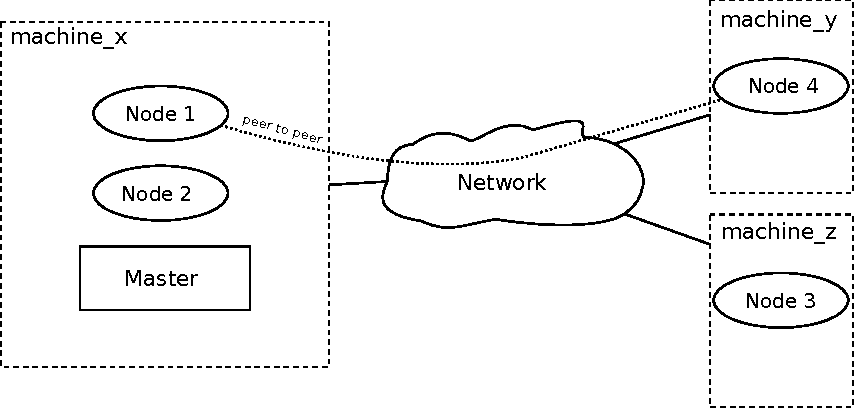
\includegraphics{./graphics/ros_components}}
  \end{center}
  \caption{Beispielhafte Ausführung von ROS auf unterschiedlichen Rechnern}
  \label{fig:roscomponents}
\end{figure}

Im Zentrum von ROS steht der sogenannte \textit{master}. Dieser wird als
einzelne Instanz gestartet und wartet dann darauf, dass sich tools, die im
Kontext von ROS gestartet werden, bei ihm anmelden. Ein als Prozess gestartetes
tool wird dabei innerhalb von ROS als \textit{node} bezeichnet. Ist der
\textit{master} nicht gestartet, können auch keine \textit{nodes} gestartet
werden. Die \textit{nodes} sind also alle zunächst auf Kommunikation mit dem
\textit{master} angewiesen. Diese Kommunikation kann lokal oder nichtlokal
ausgeführt werden, d.h. der \textit{master} kann sich auch auf einem anderen
Rechner als der \textit{node} befinden, solange eine http Verbindung zwischen
beiden hergestellt werden kann. Denn das Anmelden des \textit{nodes} beim
master erfolgt über einen \gls{XML-RPC}, getragen vom http. Für den 
Softwareentwickler auf Anwendungsebene ist diese Kommunikation zur Anmeldung allerding
vollständig durch die ROS API gekapselt und er muss sich in dieser Hinsicht
nicht explizit um Verbindungsaufbau oder Nachrichtenaustausch kümmern. Wie in
der \autoref{fig:roscomponents} dargestellt, können auch die nodes
untereinander auf unterschiedlichen Rechnern ausgeführt werden. Diese zentrale
Fähigkeit von ROS lässt sich beispielsweise vorteilhaft ausnutzen durch:

\begin{itemize}
  \item Verteilung oder Auslagerung rechenintensiver \textit{nodes} auf potente Hardware
  \item Zusammenführenung von an unterschiedlichen Stellen gewonnener Daten.
\end{itemize}

So muss beispielsweise ein mobiler Roboter Bilderkennungs Aufgaben nicht selbst
ausführen, sondern kann diese an einen \textit{node} weiterleiten der auf einem
Rechencluster ausgeführt wird. Der zweite Punkt, also das Zusammenführen von
Daten ist auch besonders im Bezug auf diese Arbeit wichtig, da Pfaddaten des
Roboters und der zu testenden Sensorknoten für \textit{Pathcompare} verfügbar
gemacht werden müssen.  Die Kommunikation zwischen nodes erfolgt über
sogenannte \textit{messages}, diese enthalten die serialisierte Form der zu
übertragenden Daten. ROS bietet in seinen Kernpakten bereits zahlreiche
Definitionen für unterschiedliche \textit{message} Typen, aber es ist auch
möglich eigene zu generieren und dies wird von zahlreichen Paketen getan, um
Daten maßgeschneidert übertragen zu können. Einmal definierte \textit{message}
Typen können wiederum rekusiv in anderen \textit{message} Typen verwendet
werden. Ein Beispiel für eine message ist in \autoref{lst:transform}
dargestellt. Dieser Typ von message ist standardmäßig in ROS definiert.
Sie besteht wie erkennbar aus den zwei Typen \textit{Vector3} und
\textit{Quaternion}. Letzterer beschreibt die Rotation und der erste die
Translation. Zusammengefügt ergibt dies eine Transformationsnachricht.

\begin{lstlisting}[caption=ROS transformation message, label=lst:transform]
geometry_msgs/Vector3 translation
  float64 x
  float64 y
  float64 z
geometry_msgs/Quaternion rotation
  float64 x
  float64 y
  float64 z
  float64 w
\end{lstlisting}

Soll ein \textit{node} seine \textit{messages} anderen \textit{nodes} senden
können, so muss er dies zunächst durch festlegen einer sogenannten
\textit{topic} beim \textit{master} anmelden. Über den \textit{master} wird
dadurch diese \textit{topic} für andere \textit{nodes} im ROS sichtbar. Eine
\textit{topic} ist definiert durch eine sogenannte \textit{topic-id}, einem
eindeutigen String. Dieser ist vergleichbar mit einer URL und dient zur
Identifikation innerhalb des ROS. Eine weitere festgelegte
Eigenschaft einer \textit{topic} ist der Typ, der über sie versendeten
\textit{messages}. \textit{Nodes} welche \textit{messages} einer
\textit{topic} empfangen sollen, müssen diese \textit{topic} dann beim
\textit{master} abbonieren. Der \textit{master} vermittelt dann eine
peer-to-peer Verbindung zwischen dem Anbieter node der topic und dem
Abbonenten. Generell gilt dabei, dass topics einen unidirektionalen
Kommunikationsweg darstellen, denn es werden nur vom Anbieter aus messages
gesendet, der oder die Abbonenten der topic sind reine Empfänger. 
In programmatischer Hinsicht wird beim Empfang neuer Nachrichten innerhalb des
\textit{nodes} eine festgelegte callback Methode aufgerufen, um die
\textit{messages} zu bearbeiten. Treffen dabei Nachrichten mit einer höheren
Frequenz ein, als abgearbeitet werden können, so kommt es irgendwann zu
Verlusten, wenn die Größe der \textit{message queue} beim Empfänger überschritten
wird. Die größe dieser queue kann jedoch durch die ROS API gesteuert werden.  

Zwei weitere wichtige Begriffe in ROS betreffen die Organisierung der
Dateien die zu den einzelnen tools gehören. Dies sind:

\begin{itemize}
  \item package
  \item stack
\end{itemize}

Ein \textit{package} beinhaltet den Code, Libraries sowie die ausführbare Datei
eines tools bzw. \textit{nodes}.  In ROS sind für packages bestimmte
Ordnerstrukturen und Dateien festgelegt sodass mithilfe der von ROS
mitgebrachten tools \textit{packages} leicht gebaut, gesucht und gestartet
werden können. Beispielsweise basiert das ROS build System auf cmake und so ist
eine vorkonfigurierte cmake-Buildatei, genannt \textit{CMakeLists.txt}, in jedem
\textit{package} grundsätzlich enthalten. Eine Zusammenfassung mehrerer
\textit{packages} wird als \textit{stack} bezeichnet. 

Überträgt man die vorgestellten ROS Begriffe auf Pathcompare so ist
dieses tool, während der Ausführung,
ein einzelner \textit{node}, welcher \textit{topics} abbonieren kann, um
\textit{messages} zu empfangen. Es wird im Teil Implementierung darauf
eingegangen, welche \textit{messages} das genau sind. Alle zum Kompilieren und
Ausführen nötige Dateien sind dabei in zwei \textit{packages} namens
\textit{pathcompare} und \textit{pathcompareplugins} aufgeteilt.

\subsection{Qt}

\textit{Pathcompare} ist darauf ausgelegt alle Informationen für den Nutzer in
einer Benutzeroberfläche (fortan als GUI bezeichnet) zu visualisieren.
Da die Anbindung an ROS über C++ erfolgt, lag nahe auch die GUI in C++
umzusetzen. Dazu wurde das Qt Framework gewählt. Qt ist in C++ implementiert, wobei
allerdings auch Anbindungen für zahlreiche andere Sprachen wie z.B.
Java, C\#, Ruby oder Python existieren. Die Entwicklung von Qt begann 1991 und
%TODO Quelle anbringen
%http://my.safaribooksonline.com/0131872494/pref04?portal=oreilly#X2ludGVybmFsX0ZsYXNoUmVhZGVyP3htbGlkPTAxMzE4NzI0OTQveGlpaQ==
ist zum Zeitpunkt des Schreibens in der Version 4.7.4 verfügbar. Das Framework besteht dabei
mittlerweile nicht mehr nur aus reinen GUI Bibliotheken, sondern stellt auch
z.B. Netzwerk-, SQL- und andere Anwendungs-Bibliothken zur Verfügung.

Ein entscheidender Vorteil des Qt Frameworks ist die gebotene große
Plattformunabhängigkeit.
Gleichzeitig wird für alle unterstützten Betriebssysteme, deren nativer Look\&Feel
verwendet. Gleicher Look\&Feel bedeutet dabei, dass das Erscheinungsbild von GUI Elementen der
Qt Anwendung dem Erscheinungsbild von GUI Elementen des Betriebssystems
gleicht.
Für die Entwicklung von \textit{Pathcompare} waren neben den GUI Bibliotheken
und schon genannten Vorteilen,
besonders folgende Konzepte und Funktionen beim Entwickeln von Nutzen: 

\begin{itemize}
  \item Signal-Slot Konzept
  \item Plattformunabhängigkeit
  \item graphischer GUI Designer 
  \item Containerklassen mit praktischen Hilfsmethoden
\end{itemize}

Auf einige dieser Punkte und deren Bezug zu Pathcompare wird nun kurz eingangen.

Das \textit{Signal-Slot} Konzept dient dazu, bestimmte Veränderungen an
Objekten, beobachtenden Objekten mitzuteilen.  Es realisiert also das
Entwurfsmuster des \textit{Observer patterns}.  \textit{Signal-Slot} erspart es
dem Programmierer einen Verweis auf das beobachtende Objekt, durch einen
registrierenden Methodenaufruf beim aktualisierenden Objekt, zu hinterlegen.
Das erleichtert den Entwicklungsprozess, da nicht mehr explizite Methoden zum
Registrieren von Beobachtern definiert werden müssen.  Stattdessen emittiert,
im Falle einer mitzuteilenden Aktualisierung, das aktualisierende Object ein
sogenanntes Signal, welches durch einen Qt Makro als \textit{signal}
ausgezeichnet ist. Bei Beobachter Objekten, die auf dieses Signal reagieren
sollen, wird dann eine als \textit{slot} deklarierte Methode selbständig
aufgerufen, sofern die Objekte, durch einen vorhergegangenen Aufruf, einer von
Qt bereitgestellten, statischen connect Methode, verbunden wurden. Wie bereits
angesprochen erhöht dieses Konzept, durch Wegfall der manuellen Implementierung
von Beobachter Registriermethoden die Flexibilität für den Entwickler deutlich.
Allerdings ist der durch Qt gekapselte Code, welcher durch Auflösung der Makros
und Kompilierung entsteht, aufblähend und dadurch langsamer bei der Ausführung
als eine direkte Implementierung mit Beobachter Registriermethoden. In der
Praxis ist diese Verlangsamung aber unmerklich und wiegt nicht die Vorteile für
den Entwickler auf. Deshalb wurde das Konzept auch bei der Entwicklung von
\textit{Pathcompare} eingesetzt. 

Im Zusammenhang mit dem Signal-Slot Konzepts wurde bereits erwähnt, dass Qt C++
um verschiedenen Makros erweitert. Diese Makros werden dabei nicht immer direkt
in gültigen C++ Code übersetzt, sondern dienen als Annotationen. Dies hat
Folgen für den Build Vorgang, denn die mit Annotationen versehenen Klassen
müssen zuerst, mit dem von Qt bereitgestelltem, \gls{MOC} übersetzt werden.
Durch den MOC wird aus den mit Annotationnen versehenem C++ Code, erneut C++
Code erzeugt, der anschließend durch normale Compiler übersetzt werden kann.
Standardmäßig wird in \textit{Qt} das Build Programm qmake verwendet, welches
die nötigen Aufrufe des \gls{MOC} automatisch veranlasst. In Hinblick auf
\textit{Pathcompare} war aber eine Integration in das von ROS genutzte Build
verfahren cmake notwendig. Hierbei muss beachtet werden, dass cmake die Dateien
welche einen \gls{MOC} Aufruf notwendig machen, in der derzeitigen Version,
nicht selbständig erkennt. Diese müssen manuell in der
Buildkonfigurationsdatei, genannt \textit{CMakeLists.txt}, deklariert werden.
Eine solche CMakeLists.txt Datei ist in jedem ROS package vorhanden und muss
für diese angepasst werden. Die sonstige Einbindung \textit{Qt} spezifischer
Libraries und deren Verlinkung mit der Applikation ist in cmake in wenigen
Zeilen deklariert. Somit war insgesamt die Verwenung von Qt in
\textit{Pathcompare} kein Hindernis für die Verwendung von cmake. Die Nutzung
von cmake wird darüberhinaus, für große Projekte, von der Qt Dokumentation
selbst empfohlen.
%TODO Quelle Doku Eintrag anbringen?

Neben dem \gls{MOC} existiert noch ein sogenannter \gls{UIC}. Dieser tritt im
Zusammenhang mit dem graphischen GUI Designer in Erscheinung. Dieser wird
\textit{QtDesigner} genannt. Beim Erstellen einer GUI mit diesem, wird eine
spezielle XML Datei vom Designer erstellt, welche den Aufbau der GUI abbildet.
Der UIC ist dann dafür verantwortlich diese Datei in C++ Klassen zu übersetzen.
Auch hier muss cmake veranlasst werden zunächst für einen \gls{UIC} Aufruf
entsprechender Dateien zu sorgen.

%TODO Quelle Plug-in Seite anbringen?

\section{Design der Software}
Wie bereits im Abschnitt ``Aufgabenstellung'' erwähnt, lag der Hauptfokus beim
Design der Pathcompare GUI darauf, einfache Benutzung und übersichtliche
Darstellung der Informationen, für den Nutzer, zu gewährleisten.  Außerdem
sollte die Software leicht erweiterbar sein, um flexiblel auf neue
Testbedingungen oder geänderte Anforderungen reagieren zu können.
Im folgenden Abschnitt wird beschrieben, wie Pathcompare realisiert wurde um
diese Ziele umzusetzen.

\subsection{Überblick Gesamtsystem}

Im Folgendem wird die Software in einer Gesamtansicht dargestellt und
anschließend auf die Funktionsweise ihrer Einzelkomponenten genauer eingegangen.

Wie in vorherigen Teilen bereits erwähnt ist \textit{Pathcompare} durch
Plug-ins erweiterbar. Dadurch kann man zunächst das Gesamtsystem in zwei Teile
untergliedern, nämlich in 

\begin{enumerate}
  \item Rahmen
  \item Plug-ins
\end{enumerate}

Rahmen und Plug-ins sind dabei in zwei unterschiedlichen ROS packages
organisiert. Das package pathcompare beinhaltet alle den Rahmen betreffenden
Dateien und das package pathcompareplugins beinhaltet die Plug-ins.
Die Aufteilung spiegelt sich auch in der GUI wider.
Hierbei bildet die GUI des Rahmens die Grundlage für die Visualisierung von Plug-ins.
Dabei wird den Plug-ins, nachdem sie geladen wurden, ein Platz innerhalb des
Rahmens zugewiesen. Innerhalb dieses zugewiesenen Platzes können sie beliebige
eigene UI Elemente laden und haben die volle Kontrolle über diese. Insgesamt
gehören die drei folgenden GUI Elemente zum Rahmen:

\begin{itemize}
\item Hauptfenster
\item Topic Übersicht
\item Plug-in Tab-Fenster
\end{itemize}

Siehe dazu auch \autoref{fig:pathcompare}.
Das Hauptfenster dient dabei als Grundlage für die Topic Übersicht und das
Plug-in Tab-Fenster. Die Topic Übersicht und das Plug-in Tab-Fenster sind vertikal
getrennt. Die Topic-Ansicht ist dabei ganz links angeordnet, siehe   .

%TODO Gesamtansicht im Text referenzieren
\begin{figure}[t]
  \begin{center}
    \fbox{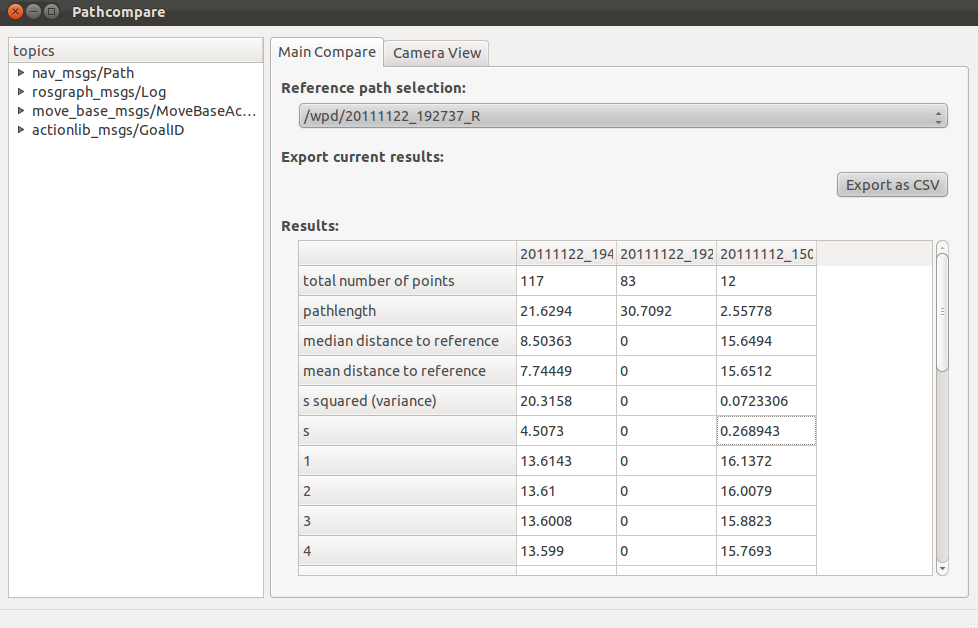
\includegraphics{./graphics/screenshotpathcompare4}}
  \end{center}
  \caption{Screenshot of Pathcompare}
  \label{fig:pathcompare}
\end{figure}

Rechts neben der Topic Übersicht schließt unmittelbar das Plug-in Tab-Fenster
an. Wird ein Plug-in geladen, wird in diesem Tab-Fenster ein neuer Tab
angelegt. Die Fläche dieses Tabs wird diesem Plug-in dann zur Verfügung
gestellt um sein UI darauf aufzubauen. Auf Details bezüglich des Ladens der
Plug-ins und deren Funktionsweise wird in einem folgendem Abschnitt ``Main
Compare'' eingegangen. 
%TODO Referenz zu Plug-in Abschnitt

Die Topic Übersicht zeigt die momentan im ROS verfügbaren Topics an. 
Um die Übersicht auf die Topics zu strukturieren ist sie derart
gestaltet, dass Topics desselben \textit{message} Typs gruppiert werden. Diese
Gruppen werden dann kompakt im Topic Übersicht Fenster angezeigt und können dort durch
den Nutzer aufgeklappt werden um alle \textit{topics} eines Typs anzuzeigen.
Dies ermöglicht es, nur solche Topics zu beobachten, die auch
tatsächlich relevant sind für den Nutzer. 
Siehe auch \autoref{fig:topics} für eine typische Ansicht der Topic Übersich mit aus- und
eingeklappten Topic Gruppen.

%TODO im Text auf topic übersicht Screenshot verweisen
\begin{figure}[t]
  \begin{center}
    \fbox{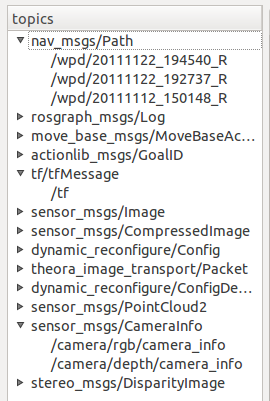
\includegraphics{./graphics/screenshottopics}}
  \end{center}
  \caption{Topic Übersich}
  \label{fig:topics}
\end{figure}

Die Platzaufteilung zwischen der Topic Übersicht und des Plug-in Tab-Fensters,
innerhalb des Hauptfensters, wurde zugunsten des Plug-in Tab-Fensters gewählt,
sodass dieses mehr Platz einnimmt.  Dies hat auch zur Folge, dass beim Vergrößern
des Hauptfensters, die Fläche des Plus-in Tab-Fensters vertikal und horizontal
vergrößert wird. Die eingenommene Fläche der Topic Übersicht wächst allerdings
nur vertikal wesentlich an. Diese Designentscheidung begründet sich darin,
dass die Plug-ins den wesentlichen Inhalt für den Nutzer präsentieren. Die
Topic Übersicht wird hingegen vermutlich nur kurzzeitig betrachtet werden und
liegt nicht im Zentrum des Interesses. Darüber hinaus ist die Topic Übersicht
sehr kompakt gestaltet und der horizontale Platzbedarf fällt gering aus.


\subsection{Anbindung an ROS}

Die Hauptaufgabe des Rahmens ist es eine Anbindung an ROS zu gewährleisten.
Diese Anbindung muss es den Plug-ins ermöglichen, benötigte \textit{topics} zu
abbonieren. Für diese Anbindung ist in \textit{Pathcompare} die Klasse
\textit{ROSManager} verantwortlich. Im Konstruktor dieser Klasse wird durch
entsprechende ROS API Aufrufe der \textit{node} \textit{pathcompare}
erstellt. Dies geschieht durch starten eines separaten Threads, da der ROS Code
in einer eigenen while-Schleife ausgeführt werden muss, die über die gesamte
Lebenszeit des \textit{nodes} bearbeitet wird. Innerhalb dieser Schleife wird
beispielsweise, das eintreffen neuer \textit{messages} von abonnierten
\textit{topics} abgearbeitet.
Zugriff der Plug-ins auf ROS spezifische Funktionalität wird komplett über den
\textit{ROSManager} gekapselt. Diese Zentralisierung ist deshalb nötig, umd den Zugriff
der verschiedenen Plug-ins, auf ROS, zu koordinieren. 
Die wichtigste Methode \textit{subscribeToTopic()}, die durch den ROSManager den Plug-ins zur
Verfügung steht, ermöglicht es eine als Parameter übergebene \textit{topic} zu
abbonieren. 


Beim Abonnieren einer \textit{topic} wird in ROS typischerweise direkt eine
Methode als Callback angegeben, welche eingehende \textit{messages} bearbeitet.
Bei einer einfachen Abbonierung ist es dabei zunächst nicht möglich mehrere
Callbacks zu registrieren.
In \textit{Pathcompare} bestehtehen in dieser Hinsicht allerdings zwei
Schwierigkeitn denen bei der Entwicklung begnet werden musste:

\begin{enumerate}
  \item eventuell abbonieren mehrere Plug-ins eine topic
  \item topics können von beliebigem \textit{message} Typ sein
\end{enumerate}

Gelöst wurde das Problem durch die Verwendung von
\textit{ros::message\_filter::cache}. Objekten dieser Klasse wird bei der
Initialisierung eine \textit{topic} zugewiesen. Empfangene \textit{messages}
dieser \textit{topic} werden in einem Ringpuffer mit einstellbarer größe
Zwischengespeichert.  Außerdem erlaubt diese Klasse die Registrierung beliebig
vieler Callbacks.  Der \textit{ROSManager} sorgt also dafür, dass für jede von
den Plug-ins benötigte \textit{topic} genau ein
\textit{ros::message\_filter::cache} Objekt existiert. Plug-ins erhalten dann
einen Verweis auf dieses Objekt und können ihren Callback registrieren. Siehe
dazu auch \autoref{fig:rosmanager}.
\autoref{fig:rosmanager} ist ein Beispiel für eine Ausführung von Pathcompare
in Verbindung mit drei Plug-ins. Über das ROS werden die drei topics topic\_x,
topic\_y und topic\_z angeboten. Durch einen Aufruf von der subscribe Methode
des ROSManager möchte Plug-in 1 die topic x abbonieren. Der ROSManager legt aus
diesem Grund einen cache an und gibt an das Plug-in 1 einen Verweis darauf
zurück. Plug-in 2 möchte dieselbe topic abbonieren und erhält ebenfalls einen
Verweis auf denselben cache. Plug-in 3 verlangt jedoch die topic\_y zu
abbonieren und es erfolgt das anlegen eines neuen caches. 

\autoref{fig:rosmanager}.

\begin{figure}[t]
  \begin{center}
    \fbox{
\includegraphics{./graphics/rosmanager}}
  \end{center}
  \caption{Anbindung an ROS durch ROSManager}
  \label{fig:rosmanager}
\end{figure}

Weitere Methoden die der ROSMaster den Plug-ins zur Verfügung stellt, dienen
beispielsweise dazu, den Plug-ins mitzuteilen, welche topics momentan im ROS
verfügbar sind. Für eine komplette Übersicht sei an dieser Stelle auch auf die
Klassendefinition rosmanager.h, die im package pathcompare zu finden ist,
verwiesen.

Die Klasse \textit{ROSManager} sorgt außerdem dafür, dass die Topic Übersicht
regelmäßig aufgefrischt wird. Es wird also dem Nutzer ersichtlich, sollten neue
\textit{topics} erscheinen oder wenn diese nicht mehr verfügbar sind.  Da die
ROS \gls{API} keinen event service anbietet um Beobachter zu benachrichtigen,
falls sich der Status von \textit{topics} ändert, stellt der
\textit{ROSManager} sekündlich eine Anfrage an den \textit{master} nach dem
aktuellen Stand der topics.  Dies ist gesteuert über einen QTimer in Verbindung
mit dem Signal-Slot Konzept.

\subsection{Laden von Plugins}
Das Einbinden von Plugins in den Rahmen steuert die Klasse
\textit{PluginLoader}. Sie sucht dabei in einem Verzeichnis nach als Plug-in
infrage kommenden Dateien. Bei dieser Suche werden generell nur shared Library
Dateien betrachtet. Handelt es sich um eine für \textit{Pathcompare} gültige
Plug-in Datei, fragt der \textit{PluginLoader} zunächst den Namen des Plug-ins
über eine im Plug-in Interface spezifizierte Methode \textit{getName()} ab.
Anschließend wird im Plug-in Tab Fenster ein neuer Tab angelegt. Dabei wird im
Tab Reiter der erfragte Name des Plug-ins eingetragen. Dadurch sind in der GUI
die Plug-ins für den Nutzer leicht zu unterscheiden und können schnell
angewählt werden.  Der Plug-in Ordner steht während der Laufzeit von
\textit{Pathcompare} unter der Beobachtung des \textit{PluginLoaders}.  Obwohl
\textit{Pathcompare} bereits gestartet wurde, können also Plug-ins in das
Plug-in Verzeichnis eingefügt werden und diese werden geladen. Dies bietet mehr
Flexibilität für den Nutzer und Entwickler, da kein Neustart der Rahmen
Anwendung sowie der ausgeführten \textit{Plug-ins} erforderlich ist.

\subsection{Main Compare Plug-in}
\label{sub:maincompare}


\textit{Main Compare} implementiert die eigentliche Hauptfunktionalität um Pfaddaten des
Referenzsystems und der Sensorknoten zu vergleichen und auszuwerten. 
Es ist dabei der Philosophie von \textit{Pathcompare} folgend auch als Plug-in
implementiert worden, welches beim Starten des Rahmens durch den
\textit{PluginLoader} geladen und ausgeführt wird.

In der GUI werden dem Nutzer verschiedene Informationen sowie
Einstellungsmöglichkeiten bezüglich der
empfangenen Pfaddaten angezeigt. Die Funktionen der einzelnen GUI Elemente
werden im Folgenden aufgezeigt.
Insgesamt gibt es drei Bereiche in der GUI, welche sich anhand dreier
verschiedener Labels abgrenzen lassen. Von oben nach untern gesehen sind
dies die Bereiche:

\begin{enumerate}
  \item Reference path selection
  \item Export results
  \item Results
\end{enumerate}

%TODO verweis auf screenshot des Plugins einfügen
%screenshot des Plugins

Der Bereich der ``Reference path selection'' beinhaltet eine Combo-Box, welche
alle über ROS verfügbaren \textit{topics} des Typs nav\_msgs/Path beinhaltet.
Der Nutzer kann dann aus dieser Liste einen Pfad auswählen, der als
Referenzpfad genutzt werden soll. Das bedeutet, dass der ausgewählte Pfad als
Referenz für die übrigen Pfade gilt. So werden dann die Abstandsberechnungen
bezüglich dieses Pfades durchgeführt. Die Auswahl des Referenzpfades kann
jederzeit geändert werden, und die Abstände werden stets neu berechnet.

Unterhalb des ``reference path selection'' Bereichs befindet sich der ``Export
results'' Bereich. Er dient dem Nutzer dazu, die berechneten und
im ``Results'' Bereich visualisierten Ergebnisse, permanent zu speichern.
Die Speicherung erfolgt dabei als \gls{CSV} Datei. Der Export wird durchgeführt
wenn der Nutzer den in diesem Bereich vorhandenen Button drückt. 
Das genaue Format der gespeicherten Daten wird später erläutert.
%TODO verweis auf den Abschnitt ``format CSV Datei'' anbringen 

Der ``Result'' Bereich dient dazu alle ermittelten Informationen bezüglich der
Pfade, für den Nutzer anzuzeigen. Die Visualisierung erfolgt hierbei durch eine
Tabbellenstruktur. In dieser Tabelle wird für jede Path topic ein Spalte
angelegt.
In jeder Zeile einer Spalte sind dabei die unterschiedlichen
Informationen eingetragen.
Main Compare verhält sich außerdem so, dass topics, welche einmal in
der Tabelle erfasst wurden auch dort verbleiben. Sollte also eine topic nicht
mehr im ROS zur verfügung stehen, bleiben die angezeigten Informationen auf
Basis der zuletzt empfangenen Werte dennoch erhalten. 

In der Tabelle werden für den Nutzer folgende Informationen:
angezeigt:

\begin{itemize}
  \item Anzahl der Lokalisierungen
  \item Berechnung der Pfadlänge
  \item Anzeige des Medians der Abstände
  \item Anzeige des arithmetischen Mittels der Abstände
  \item Berechnung der empirische Varianz $s^2$ der Abstände
  \item Berechnung der empirische Standardabweichung $s$ der Abstände
  \item 20 größten Abstände zu Referenzpfad
\end{itemize}

Die angezeigten Informationen werden bei Empfang neuer Pfad \textit{messages} stets
aktualisiert. Generell gilt dabei, dass jede Path message den kompletten Pfad
enthalten muss. Pfade können also nicht stückweise übertragen werden. Dieses vorgehen
bietet die Möglichkeit, dass Pfaddatenen nachträglich geändert werden können.
Also kann beispielsweise die erste Lokalisierung innerhalb eines Pfades zu einem
späteren Zeitpunkt abgeändert werden. 

Um nachzuvollziehen wie die in Main Compare angezeigten Informationen ermittelt werden, bietet
es sich an, zunächst den Typ der \textit{messages}, welche über die Pfad topics
empfangen werden, zu analysieren. Denn auf dieser Basis leiten sich alle
ermittelten Informationen ab. Wie bereits beschrieben sind die messages vom Typ
\textit{nav\_msgs/Path}, der wie folgt definiert ist:

\begin{lstlisting}[caption=ROS transformation message, label=lst:pathmsgs]
Header header
  uint32 seq
  time stamp
  string frame_id
geometry_msgs/PoseStamped[] poses
  Header header
    uint32 seq
    time stamp
    string frame_id
  geometry_msgs/Pose pose
    geometry_msgs/Point position
      float64 x
      float64 y
      float64 z
    geometry_msgs/Quaternion orientation
      float64 x
      float64 y
      float64 z
      float64 w
\end{lstlisting}

Zunächst ist in \autoref{lst:pathmsgs} zu erkennen, dass sich dieser \textit{message} Typ aus anderen Typen
zusammensetzt. Auf der obersten Ebene ist dies ein
\textit{Header} und ein Array von \textit{geometry\_msgs/PoseStamped}.
Der Header dient dazu, die Path message von anderen empfangenen
Path messages zu unterscheiden und dazu die messages ordnen zu können. Die Ordnung kann dabei über eine Sequenznummer
(seq) oder einen Zeitstempel (stamp) hergestellt werden. Das Feld frame\_id
definiert einen Bezugsrahmen innerhalb von ROS, es wird aber im Kontext von
Main Compare nicht ausgewertet und wird hier deswegen nicht genauer erläutert.
Die eigentlichen Pfaddaten verbergen sich in dem Array von PoseStamped. Auch
PoseStamped ist ein zusammengesetzer Typ, bestehend aus einem Header und einer
Pose. Die Pose setzt sich aus einem Point und einer Quaternion zusammen.
Der gefahrende Pfad wird nun dadurch in der Path message abgebildet, indem bei
jeder durchgeführten Lokalisierung eine PoseStamped angelegt wird. Diese PoseStamped
hält im Header die Zeit der Lokalisierung und eine Sequenznummer fest. In der
Pose wird dann der bei der Lokalisierung ermittelte Punkt, als Point eingetragen. Die Quaternion
hält fest, welche Ausrichtung dabei im Raum vorliegt und wird auch
in die Pose eingefügt. Die Ausrichtung ist
allerdings optional und wird in der derzeitigen Version von Main Compare nicht beachtet. 
Außerdem lässt sich in \autoref{lst:pathmsgs} erkennen, dass die
Lokalisierungen dreidimensional erfolgen können. Die von Main Compare
ausgeführten Berechnungen sind aber auch mit Daten niederer Dimension möglich,
indem die nicht genutze Dimension auf 0 gesetzt wird. Beispielsweise werden,
in der derzeitigen Form des Referenzsystems, vom Roboter zweidimensionale
Lokalisierungsdaten in der x-y Ebene übermittelt und die z Komponente erhält
immer den Wert 0. Wie schon in Bezug auf die orientation erwähnt, werden nicht alle Komponenten der
Pfad message in Main Compare verwendet. Für die derzeitige Version sind
folgende Felder relevant:

\begin{itemize}
  \item poses.stamp (Typ ros::time)
  \item pose.position.x (Typ float64)
  \item pose.position.y (Typ float64)
  \item pose.position.z (Typ float64)
\end{itemize}

Obwohl nicht alle Felder der Path message genutzt werden, ist dieser message Typ
für Main Compare die geeignete Wahl, da er in ROS standardmäßig
definiert ist, was die Definition und deren Verteilung, eines
eigenen message Typs, vermeidbar macht. Außerdem sind die ungenutzen Felder nicht
übermäßig groß und werden die Kapazitäten des Übertragungskanals kaum belasten.
Vernachlässigt man die ungenutzten Felder des Header, der eine in ROS definierte Standardmessage ist, fallen nur
zusätzliche 24 Byte für die ungenutze orientation, pro übertragenem Point, an.
Darüberhinaus ist es denkbar, dass die orientation in späteren Versionen von
Main Compare doch noch betrachtet wird und somit die durchzuführenden
Änderungen klein ausfallen.

Anhand der oben aufgezählten, genutzen Felder, lässt sich ein Pfad abstrakt durch eine Menge
$M$ von Tupeln modellieren. Dabei setzen sich die Tupel aus einem Zeitstempel und einem dreidimensionalem
Punkt zusammen. In Anlehnung an die verwendeten Bezeichner in
\autoref{lst:pathmsgs}, sei $M$ demnach wie folgt definiert:

\begin{equation*}
  \label{eqn:setdef}
  M := \{ (p.stamp , p.position) \mid p \in poses \}
\end{equation*}

Die konkrete Repräsentierung dieses Modells erfolgt in Main Compare durch die
Klassen \textit{TopicPath} und \textit{Position}. TopicPath repräsentiert dabei
die Menge $M$. Position repräsentiert ein einzelnes Tupel und enthält somit den
Zeitstempel und zugehörigen Punkt. Dem Modell entsprechend enthält ein
TopicPath Objekt eine Liste von Position Objekten.  Neben den Klassen TopicPath
und Position gibt es noch eine Klasse \textit{TopicPathManager}. Es wird genau
ein Objekt dieser Klasse für jede im ROS verfügbare Path topic angelegt. Diese
Klasse bietet eine callback Methode, welche beim, zur topic gehörenden,
message\_filter::cache registriert wird. Kommt eine neue message an, wird die
callback Methode aufgerufen und aus den Werten der Path message ein neues
TopicPath Objekt erstellt. Anschließend werden, anhand des neuen TopicPaths,
alle nötigen Berechnungen erneut durchgeführt und die Results Tabelle
aktualisiert. Die Beziehung der Klassen Position, TopicPath und
TopicPathManager werden in \autoref{fig:topicpathrelated} verdeutlicht.

\begin{figure}[t]
  \begin{center}
    \fbox{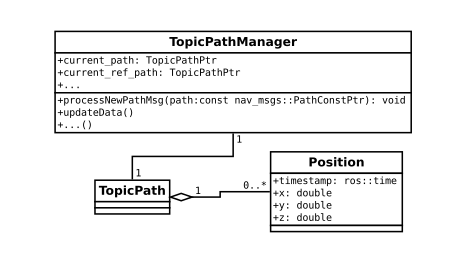
\includegraphics{./graphics/topicpathrelated}}
  \end{center}
  \caption{In Main Compare verwendete Klassen zum verarbeiten von Pfaden}
  \label{fig:topicpathrelated}
\end{figure}

Anhand der abstrakten Modellierung $M$ eines Pfades, werden im Folgenden, die von
Main Compare ausgeführten Berechnungen erläutert. In der konkreten
Repräsentatio erfolgen alle Berechnungen in der Klasse \textit{TopicPathManager}. 

\subsubsection{Anzahl der Lokalisierungen}
Um die Anzahl der Lokalisierungen zu ermitteln wird in Main Compare lediglich die
Mächtigkeit der Menge $M$ bestimmt. Es gilt also:

\begin{equation*}
  \label{eqn:numofpoints}
  number of points = \vert M \vert
\end{equation*}

Im \textit{TopicPathManager} ist dies entsprechend einfach realisiert.
%Siehe dazu TopicPathManager::

\subsubsection{Berechnung der Pfadlänge}
Bei der Bestimmung der Pfadlänge werden zunächst alle Abstände, zwischen je
zwei direkt aufeinanderfolgenden Punkten im Pfad, bestimmt. Die Summe all dieser
Abstände entspricht dann der Gesamtlänge des Pfades. Dazu muss jedoch noch
geklärt werden, wann ein Punkt $p_1$ in einer Path message auf einen anderen
Punkt $p_2$ folgt. Das lässt sich über den Zeitstempel feststellen und ist
anschaulich ausgedrückt dann der Fall, wenn keine weitere Lokalisierung in
der Zeit zwischen der Lokalisierung $p_1$ und $p_2$ stattgefunden hat. Dies kann man auch wie
folgend, abstrakt und bezogen auf $M$, ausdrücken.  Ein Punkt $p_2$ ist direkt
folgend auf einen Punkt $p_1$, genau dann wenn für die zugehörigen Tupel

$t_1 := (z_1, p_1)$ und $t_2 := (z_2, p_2)$
mit
$t_1,t_2 \in M$
gilt, dass:
\[
z_2 > z_1 \wedge \nexists (z^{,}, p^{,}) \in M : z_2 > z^{,} > z_1
\]

Der Abstand zweier aufeinanderfolgender Punkte lässt sich einfach durch
Vektorsubtraktion und anschließende Betragsbildung des resultierenden Vektors
bestimmen.
%TODO Siehe dazu TopicPathManager::

\subsubsection{Pfadvergleichsverfahren und Abstandsberechnung}

Das Hauptziele von Main Compare ist es, dem Nutzer zu erleichtern, die
Genauigkeit eines durch Lokalisierung gewonnenen Pfades, in Bezug auf einen
Referenzpfad, abzuschätzen. Um dies zu tun, ist es notwendig, den Abstand von
Lokalisierungen des zu untersuchenden Pfads, zu denen des Referenzpfads, zu
ermitteln. In einem naiven Ansatz, um diesen Abstand zu bestimmen, könnte man die Lokalisierungen direkt
miteinander vergleichen. Unter der Voraussetzung, dass für jeden Punkt des Referenzpfades auch
ein Punkt im zu vergleichenden Pfad mit demselben Zeitstempel existiert. Der
Vergleich zwischen Referenz und zu untersuchendem Pfad fällt dann denkbar einfach aus, denn man müsste nur den Abstand je
zweier Punkte, mit demselben Zeitstempel, bestimmen.
Das Problem bei dieser Methode ist jedoch, dass das Referenzsystem und die
einzelnen Sensorknoten unabhängig voneinander sind und dadurch Lokalisierungen
nicht immer zum selben Zeitpunkt oder mit einer anderen Frequenz durchführen 
können. Um dies zu verhindern müsste man wie in Abb. gezeigt einen zentralen
Taktgeber in das System integrieren, der durch ausgesendete Impulse, zum
Beispiel in der Form einer ROS message, den Komponenten vorschreibt,
wann eine Lokalisierung durchgeführt werden soll.
%TODO bild test mit Tickgeber
Die Einführung eines solchen Taktgebers verkompliziert jedoch die
Testausführung und setzt bei allen am Test beteiligten Komponenten voraus, dass
deren Software auf diesen Mechanismus reagiert. Zudem ist man während des Tests
zwingend auf eine ungestörte Netzwerkkommunikation angewiesen, da sonst der
Impuls nicht gleichmäßig oder gar nicht bei den Komponenten ankommt.

Aufgrund dieser schwerwiegenden Nachteile wurde bei der Entwicklung von Main
Compare ein Ansatz gewählt, der es den Komponenten erlaubt Lokalisierungen zu
beliebigen Zeitpunkten und mit beliebiger Frequenz durchzuführen. Die einzige
Voraussetzung ist dabei, dass die Uhren der Komponenten, mit einem gewissen
tollerierbaren Fehler, synchronisiert werden. Dies sichert, dass die Zeitstempel der
Lokalisierungen zuverlässig vergleichbar sind. Der Abstand wird wie folgt
ermittelt, siehe dazu auch Abb. . Für jeden Punkt im zu vergleichenden Pfad $A$
%TODO bild variante ohne tick
wird der Abstand zum Refernzpfad $R$ bestimmt. Dazu wird der jeweilige
Zeitstempel $z_a$ eines Punktes $p_a$ aus A einem passenden
Zeitstempelintervall zweier aufeinanderfolgender Punkte $p_{r2}$ , $p_{r1}$ aus $R$ zugeordnet, sodass
gilt:
\[
z_{r1} <= z_a < z_{r2}
\]

Ist dieses Intervall gefunden, wird der Abstand von $p_a$ zum Geradensegment
$\overline{p_{r2} p_{r1}}$ bestimmt. Um diesen Abstand zu bestimmen wird das
Lot auf die von $p_{r1}$ und $p_{r2}$ bestimmte Gerade ermittelt. Fällt das Lot
dabei zwischen $p_{r1}$ und $p_{r2}$ auf die Gerade wird der Abstand vom
Lotpunkt zu $p_a$ errechnet. Fällt er jedoch außerhalb dieses Intervalls muss
der Abstand, je nach Lage des Lotpunkts, entweder zu $p_{r1}$ oder $p_{r2}$
bestimmt werden. Siehe dazu auch Abb. .
%TODO bild abstandsbestimmung

Charakteristisch bei dieser Art der Abstandsbestimmung ist, dass beim
Referenzpfad zwischen zwei Lokalisierungen, durch das Geradensegment, die
Position interpoliert wird. Es wird also angenommen, dass die tatsächlich
ausgeführte Bewegung zwischen den Punkten, einer Gerade entspricht. Daraus
folgt aber, dass man die Lokalisierungsfrequenz des Referenzpfades, an die
Bewegungsgeschwindigkeit des Referenzsystems anpassen muss. Dabei soll
zwischen zwei Lokalisierungen des Referenzpfades die interpolierte Strecke
klein bleiben, denn dadurch nähert sie sich stärker der tatsächlich gefahrenen
Strecke an. Betrachtet man das derzeitige Referenzsystem, mit dem TurtleBot, so
ist die Bewegungsgeschwindigkeit allerdings gering und eine sekündliche
Lokalisierung erscheint ausreichend. Dies muss jedoch noch durch weitergehende
Tests bestätigt werden.

%TODO evtl. Verweis auf TopicPathManager::   Methode

\subsubsection{Bestimmung empirischer Varianz und Standardabweichung}
Auf Basis der zuvor beschriebenen Abstandsberechnung wird in Main Compare die
empirische Varianz der Abstände bestimmt. Um diese zu berechnen wird zunächst
das arithmetische Mittel gebildet, welches ebenso in der Results Tabelle angezeigt wird.
Anschließend wird die empirische Varianz $s^2$ gebildet. Die empirische Standardabweichung
ist die Wurzel aus $s^s$ also $s$.

\subsubsection{Bestimmung des Median der Abstände}
Der Medians der Abstände, ist robuster gegenüber Ausreißern als das
arithmetische Mittel und wird deshalb ermittelt und auch in der Results Tabelle
aufgeführt.

\subsection{Das Plug-in Konzept}
Im folgenden Abschnitt wird das Konzept des Pathcompare Plug-in Mechanismus
erläutert und aufgezeigt, welche Schritte erforderlich sind, um eigene Plug-ins
für Pathcompare zu erstellen. Realisiert sind die Plug-ins in Pathcompare
mithilfe der Qt Plugin API. Diese gibt Strukturen vor, um Plug-ins zu
definieren. Außerdem beinhaltet sie Klassen, um Plug-ins während der Laufzeit
einer Applikation zu laden.  Bei Verwendung dieser API müssen, um Plug-ins zu
erstellen, im wesentlichen zwei Schritte ausgeführt werde, dies sind:

\begin{enumerate}
  \item Definition eines Interface
  \item Implementierung des Interfaces durch Plug-in
\end{enumerate}

Um eine Anwendung durch Plug-ins erweiterbar zu machen ist also zunächst erforderlich ein
Interface zu definieren. Dieses Interface legt fest, welche Methoden durch ein
Plug-in zu implementieren sind. Das Interface hat dabei
die Form einer Klassendefinition mit nur rein virtuellen Funktionen. Zusätzlich
wird diese Klassendefinition durch Qt Makros ergänzt, um es als Interface zu
markieren. In Pathcompare ist dieses Interface vorgegeben und trägt den langen
Namen \textit{ComparatorPluginFactoryInterface}. Wie die Implementierung dieses
Interfaces erfolgt, wird nun anhand eines vorhandenen Plug-ins für Pathcompare erläutert.
Dieses Plug-in trägt den Namen Camera View. In der derzeitigen Version von
Pathcompare wird es, ebenso wie Main Compare, beim Starten der Anwendung geladen.
Es dient dem Nutzer dazu ROS topics des Typs sensor\_msgs/Image zu
visualisieren. Dieser Typ von Topic wird beispielsweise innerhalb von ROS
genutzt um Kamerafeeds der Kinect zur Verfügung zu stellen. Camera View könnte also
bei einer Fahrt des TurtleBots eingesetzt werden um dem Tester ein Bild der
aktuellen Umgebung des Roboters zu vermitteln. Die Gestaltung der GUI dieses
Plug-ins fällt einfach aus. Der Nutzer kann mit einer ComboBox eine topic
auswählen. Nach der Auswahl, werden die empfangenden Bilder, der gewählten Image
topic, eingeblendet. 

\begin{figure}[t]
  \begin{center}
    \fbox{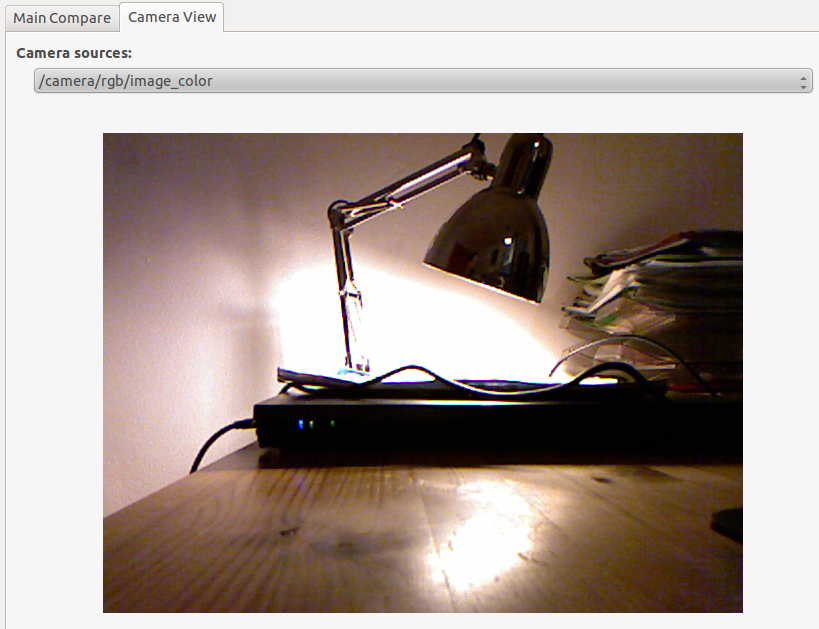
\includegraphics{./graphics/screenshotcameraview}}
  \end{center}
  \caption{GUI des Camera View Plug-ins}
  \label{fig:cameraview}
\end{figure}

Wie zuvor beschrieben muss jedes Pathcompare Plugin das Interface
\textit{ComparatorPluginFactoryInterface} implementieren, so auch Camera View.

Dieses Interface beinhaltet zwei Methoden, siehe dazu auch
\autoref{lst:factoryinterface}.

\begin{lstlisting}[caption=ROS transformation message, language=C++, basicstyle=\footnotesize, label=lst:factoryinterface]

        virtual ComparatorPluginPtr createComperatorPlugin(ROSManager * ros_manager, QWidget *tab_widget) const = 0;
        virtual QString getPluginName() const = 0;

\end{lstlisting}

Die Methode createComparatorPlugin() ist eine Factorymethode und erzeugt das
eigenliche Objekt, welches die Funktionalität des Plug-ins beinhaltet. Dieser
Umweg ist notwendig, da Plug-ins keine typischen Klassenobjekte sind. Denn bei
Qt Plug-ins handelt es sich um shared libraries. In einer shared library können
zwar Methoden ausführbar hinterlegt werden, aber kein eigenständiges Objekte
mit Attributen existieren. Der Rückgabetyp von createComparatorPlugin() ist
ComparatorPluginPtr, definiert durch \autoref{lst:returntypedef}.

\begin{lstlisting}[caption=ROS transformation message, language=C++, basicstyle=\footnotesize, label=lst:returntypedef]
//typedef for shared_ptr reference to ComparatorPlugin
typedef boost::shared_ptr<ComparatorPlugin> ComparatorPluginPtr;
\end{lstlisting}

Es handelt sich also um einen Verweis auf ein Objekt der Klasse
ComparatorPlugin. Diese Klasse ist der Basistyp, für das in der Factory Methode
dynamisch erzeugte Objekt. In Camera View ist die Factory Methode wie folgt
implementiert worden, siehe \autoref{lst:create}:

 \begin{figure}[t]
   \begin{center}
     \fbox{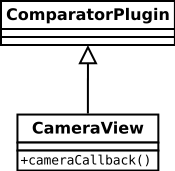
\includegraphics{./graphics/cameraviewcomparator}}
   \end{center}
   \caption{ComparatorPlugin als Basisklasse zu CameraView}
   \label{fig:cameraviewcomparator}
 \end{figure}

\begin{lstlisting}[caption=ROS transformation message, language=C++, basicstyle=\footnotesize, label=lst:create]
ComparatorPluginPtr PathcompareMainFactoryPlugin::createComparatorPlugin(ROSManager * ros_manager, QWidget *tab_widget) const
{
        ComparatorPluginPtr comp_plugin(static_cast<ComparatorPlugin *>(new CameraView(ros_manager, tab_widget)));
        return comp_plugin;
}
\end{lstlisting}

Es wird hierin ein Objekt des Typs CameraView angelegt, welches den Basistyp
ComparatorPlugin besitzt. Im Konstruktor erhält es Verweise auf den ROSManager,
welcher benötigt wird um ROS spezifische Aktionen durchzuführen. Als zweites
Konstruktorargument wird die Zeichenfläche für die Camera View GUI übergeben.
Am Ende der Methode wird das fertig angelegte Objekt zurückgegeben und steht
damit Pathcompare zur Verfügung. 

Die zweite Methode im Plug-in Interface, getName() liefert lediglich den Namen
des Plug-ins zurück und wird in Pathcompare durch die Klasse PluginLoader
genutzt.

Zusammenfassend kann man also sagen, dass die eigenlichen Pathcompare Plug-in Interface
Methoden ohne großen Aufwandt zu implementieren sind. Ein vollständiges
Referenzbeispiel zur Implementierung neuer Plug-ins ist durch Camera View gegeben.
Zu finden sind dabei alle relevanten Code- und Builddateien im Ordner
pathcompareplugins/cameraview.

